\pagebreak

\section{Xilinx Input/Output library for Virtex4 and later - xilinx/io.3pl}

    \index{library!xilinx/io.3pl}
    This library provides input and output delays and serialisers/deserialisers
    for Virtex5 and later.
    
    This library must be incorporated by using a module statement, e.g. -
    \begin{lstlisting}[gobble=4, language=threepl]
       module "xilinx/io.3pl"
    \end{lstlisting}


    \subsection{library modules}
    

        \subsubsection{crc32 - 32 bit CRC}\label{sec:lmcrc32}

            {\bf Library: xilinx/io.3pl}

            {\bf Prototype:} \\
            \vsp
            \begin{lstlisting}[gobble=12, language=threepl]
               global module
               crc32 (
                   value(out, "bits:32")
                   <-
                   value(in),
                   value(valid, "log"),
                   clock(clk),
                   value(reset, "log")
               ) {}
            \end{lstlisting}

            {\bf Output parameters:} \\
            {\bf out} CRC output.\\


            {\bf Input parameters:} \\
            {\bf in} input data.\\
            {\bf valid} data valid.\\
            {\bf clk} clock.\\
            {\bf reset} reset to CRC\_INIT initial value.\\

            {\bf description:} \\
            This module creates an interface to a CRC32 element for
            Virtex5 and later FPGAs.




        \subsubsection{crc64 - 64 bit CRC}\label{sec:lmcrc64}

            {\bf Library: xilinx/io.3pl}

            {\bf Prototype:} \\
            \vsp
            \begin{lstlisting}[gobble=12, language=threepl]
               global module
               crc64 (
                   value(out, "bits:64")
                   <-
                   value(in),
                   value(valid, "log"),
                   clock(clk),
                   value(reset, "log")
               ) {}
            \end{lstlisting}

            {\bf Output parameters:} \\
            {\bf out} CRC output.\\


            {\bf Input parameters:} \\
            {\bf in} input data.\\
            {\bf valid} data valid.\\
            {\bf clk} clock.\\
            {\bf reset} reset to CRC\_INIT initial value.\\

            {\bf description:} \\
            This module creates an interface to a CRC64 element for
            Virtex5 and later FPGAs.







        \subsubsection{dcireset - reset DCI pins}\label{sec:lmdcireset}

            {\bf Library: xilinx/io.3pl}

            {\bf Prototype:} \\
            \vsp
            \begin{lstlisting}[gobble=12, language=threepl]
               global module
               dcireset (value(locked, "log") <- value(rst, "log")) {}
            \end{lstlisting}

            {\bf Output parameters:} \\
            {\bf locked} DCI pins calibrated and available.\\


            {\bf Input parameters:} \\
            {\bf rst} calibrate DCI impedences.\\

            {\bf description:} \\
            This module creates an interface to the DCI reset hardware.
            WHen {\bf rst} is asserted (high) the DCI impedances are
            calibrated. When calibration is complete {\bf locked} will become
            true. DCI pins are unavailable during calibration.


        \subsubsection{sysmon - system monitor}\label{sec:lmsysmon}

            {\bf Library: xilinx/io.3pl}

            {\bf Prototype:} \\
            \vsp
            \begin{lstlisting}[gobble=12, language=threepl]
               global module
               sysmon (
                       value(dout, "bits:16"),
                       value(drdy, "log"),
                       value(alm, "[3]log"),
                       value(ot, "log"),
                       value(channel, "uint:5"),
                       value({eoc, eos, busy, jtaglocked, jtagmodified, jtagbusy}, "log")
                       <-
                       value(din, "bits:16"),
                       value(daddr, "uint:7"),
                       clock(dclk),
                       value({den, dwe, reset, convst, convstclk}, "log"),
                       int({   init_40, init_41, init_42,
                               init_48, init_49, init_4a, init_4b,
                               init_4c, init_4d, init_4e, init_4f,
                               init_50, init_51, init_52, init_53,
                               init_54, init_55, init_56, init_57 })
               ) {}
            \end{lstlisting}

            {\bf Output parameters:} \\
            {\bf do} reconfiguration port output data.\\
            {\bf drdy} reconfiguration port data ready.\\
            {\bf alm} temperature sensor alarm.\\
            {\bf ot} over temperature alarm.\\
            {\bf channel} current ADC channel.\\
            {\bf eoc} end of conversion.\\
            {\bf eos} end of conversion sequence.\\
            {\bf busy} ADC busy.\\


            {\bf Input parameters:} \\
            {\bf di} reconfiguration port input data.\\
            {\bf daddr} reconfiguration port address.\\
            {\bf dclk} reconfiguration port clock.\\
            {\bf den} reconfiguration port enable.\\
            {\bf dwe} reconfiguration port write enable.\\
            {\bf reset} reset.\\
            {\bf convst} convert start.\\
            {\bf convstclk} convert start clock.\\
            {\bf init\_40} to {\bf init\_57}, initial configuration data.\\

            {\bf description:} \\
            This module creates an interface to the system monitor. See
            for example Xilinx document "Virtex-5 FPGA System Monitor" UG192.



        
    \subsection{library procedures}



        \subsubsection{iddr - input double data rate interface}\label{sec:lpiddr}

            {\bf Library: xilinx/io.3pl}

            {\bf Prototype:} \\
            \vsp
            \begin{lstlisting}[gobble=12, language=threepl]
               global procedure
               iddr (
                   value(o1),
                   value(o2)
                   <-
                   value(d),
                   clock({c, cb}),
                   str(mode),
                   value({ce, r, s}, "log")
               ) {}
            \end{lstlisting}

            {\bf Output parameters:} \\
            {\bf o1} is the +ve clock edge data output.\\
            {\bf o2} is the -ve clock edge data output.

            {\bf Input parameters:} \\            
            {\bf d} is the DDR data input.\\
            {\bf c} is an optional primary clock input.\\
            {\bf cb} is an optional secondary clock input.\\
            {\bf mode} specifies the operating mode.\\
            {\bf ce} is an optional clock enable.\\
            {\bf r} is an optional synchronous reset.\\
            {\bf s} is an optional synchronous set.
        
            {\bf In-line target execution:} \\
            no

            {\bf description:} \\
            This procedure creates an input DDR (Double Data Rate) interface.
            
            The argument to input parameter {\bf d} may be an input mode
            variable or it may be the output from an interposed idelay() call.
            
            {\bf c} is an optional clock input. It is the primary or only
            clock.
            
            {\bf cb} is an optional clock input. It is a secondary clock.
            
            If neither {\bf c} nor {\bf cb} are supplied, the current clock will
            be used to capture data. If {\bf c} is supplied it will be used
            instead of the current clock. In either case both +ve and -ve edges
            of the clock are used to capture input data.
            
            If {\bf c} and {\bf cb} are both supplied {\bf c} will be used to
            capture +ve edge data and {\bf cb} will be used to capture -ve edge
            data
            
            Output parameter {\bf o1} is assigned input data clocked from the
            positive clock edges. Output parameter {\bf o2} is assigned input
            data clocked from the negative clock edges.
            
            {\bf ce} is a clock enable and controls assignment to both
            outputs.
            
            {\bf R} can be used to clear the output registers and {\bf s}
            to set them to all ones.
            
            Parameter {\bf mode} may have one of three string values -
            
            mode == "nfirst" - input data is assigned to an internal register on
            negative clock edges. Input data is assigned to {\bf o1} on positive
            clock edges. Data in the internal register is assigned to {\bf o2}
            on positive clock edges. The two outputs thus capture -ve:+ve pairs
            in that order and both outputs are clocked on the +ve clock edge.
            
            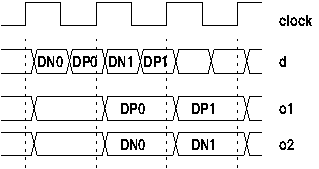
\includegraphics{iddr1}
            
            mode == "pfirst" - this is the same as above but there is an
            additional pipeline register inserted before the positive edge
            register. The two outputs thus capture +ve:-ve pairs in that order
            and both outputs are clocked on the +ve clock edge. There is an
            extra cycle of latency in this mode.
            
            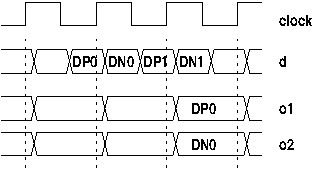
\includegraphics{iddr2}
            
            mode == "split" - input data is assigned to {\bf o1} on positive
            clock edges and to {\bf o2} on negative clock edges. The two outputs
            are thus in different (complementary) clock domains.
            
            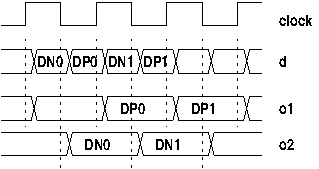
\includegraphics{iddr3}
            
            No input parameters may contain queue reads.
            
            Example code; input from a 2-channel DDR analog to digital
            converter -
            io.3pl
            \begin{lstlisting}[gobble=12, language=threepl]
               str(lvcmos33, "LVCMOS33");

               // package pins
               iopins(adc_clk_pin, lvcmos33, "str", "E17");
               iopins(adc_pins, lvcmos33, "[8]str",
                                   {"F2", "G2", "H2", "J2", "H1", "E1", "G1", "E2"});

               // ADC clock
               clock(adc_clk_in, frequency=100.0e6, loc=adc_clk_pin, ibufg=true);
               clock({global.adc_clk, adc_clk_raw}, frequency=100.0e6);
               clkdcm(clk0=adc_clk_raw <- clkin=adc_clk_in, clkfb=adc_clk);
               clockbufg(adc_clk <- adc_clk_raw);
               attributes(adc_clk, tnm="ADC_CLK");

               // ADC interface
               useclock(adc_clk);
               value({adc0, adc1}, "uint:8");
               input(adc_in, "uint:8", loc=adc_pins);
               iddr(adc0, adc1 <- adc_in,,, "nfirst");
            \end{lstlisting}
            
            Value variables {\bf adc0} and {\bf adc1} now 'point' to registers
            which are assigned ADC values on each positive edge of the clock,
            one from each channel.
            


        \subsubsection{idelay - input data delay}\label{sec:lpidelay}

            {\bf Library: xilinx/io.3pl}

            {\bf Prototype:} \\
            \vsp
            \begin{lstlisting}[gobble=12, language=threepl]
               global procedure
               idelay (
                   value(o)
                   <-
                   input(d),
                   int(delay),
                   clock(refclk),
                   value({ce, inc, rst}, "log"),
                   log(isclock)
               ) {}
            \end{lstlisting}

            {\bf Output parameters:} \\
            {\bf o} is the data output.

            {\bf Input parameters:} \\            
            {\bf d} is the data input.\\
            {\bf delay} gives a delay count.\\
            {\bf refclk} is a reference clock to control the delay.\\
            {\bf ce} is an optional clock enable for changing the delay.\\
            {\bf inc} is an optional direction control for changing the delay.\\
            {\bf rst} is an optional reset for the delay.\\
            {\bf isclock} should be true for a clock signal and false for a data
            signal.\\
         
            {\bf In-line target execution:} \\
            no

            {\bf description:} \\
            This procedure generates an input delay block.
            
            The data input {\bf d} is an input mode variable and must be a
            single bit.

            The output parameter {\bf o} is the delayed signal and is also a
            single bit.
            
            {\bf ce}, {\bf inc} and {\bf rst} inputs are used to change the
            delay value. These must be in the current clock domain.
            
            If input parameters {\bf delay} or {\bf ce} have an argument then
            the input parameter {\bf refclk} must be supplied with a clock whose
            frequency lies between 190.0MHz and 210.0MHz but is ideally 200MHz.
            If {\bf idelay()} is called more than once when {\bf variable} has
            an argument, then the same reference clock must be supplied to each
            call. Any calls to {\bf iodelay()} must also use the same reference
            clock.
            
            If input parameter {\bf ce} has no argument then the delay will be
            fixed. Input parameter {\bf delay} gives the required delay. The
            delay is $400 + 78 * delay$ pS for a reference clock frequency of
            200MHz. If {\bf delay} has no argument the delay count will be zero
            (giving $400$pS).
            
            If input parameter {\bf ce} has an argument then the delay will be
            variable. Input parameter {\bf delay} gives the initial delay count
            (default 0). The delay can be changed by asserting {\bf ce}. If {\bf
            inc} is true the delay will be incremented, otherwise it will be
            decremented. If {\bf rst} is asserted the delay will be changed back
            to the initial delay value. The clock domain of {\bf ce}, {\bf inc}
            and {\bf rst} is the current clock domain.
            
            Parameter {\bf isclock} describes the signal type which optimises
            the timing analyser for periodic or non-periodic signals.
            
            No input parameters may contain queue reads.
            
            Implementation note: this procedure will automatically create an
            IDELAYCTRL block on the first call to {\bf idelay()} that has a
            non-default delay. The Xilinx software will duplicate this across
            all locations where required. Xilinx recommend explicitly creating
            an IDELAYCTRL for each I/O region. This seems like hard work
            requiring a detailed floor plan and it is not clear why they suggest
            doing so.
            


        \subsubsection{iodelay - input/output data delay}\label{sec:lpiodelay}

            {\bf Library: xilinx/io.3pl}

            {\bf Prototype:} \\
            \vsp
            \begin{lstlisting}[gobble=12, language=threepl]
               global procedure
               iodelay (
                   value(dataout)
                   <-
                   input(idatain),
                   value(odatain),
                   log(variable),
                   int({idelay, odelay}),
                   clock(refclk),
                   value({t, ce, inc, rst}, "log")
               ) {}
            \end{lstlisting}

            {\bf Output parameters:} \\
            {\bf dataout} is the data output.

            {\bf Input parameters:} \\            
            {\bf idatain} is the data input from an IBUF (input mode variable).\\
            {\bf odatain} is the data input from OLOGIC.\\
            {\bf variable} specifies the type of input delay.\\
            {\bf idelay} gives the input delay count.\\
            {\bf odelay} gives the output delay count.\\
            {\bf refclk} is a reference clock to control the delays.\\
            {\bf t} is 3-state output control.\\
            {\bf ce} is an optional clock enable for changing the delay.\\
            {\bf inc} is an optional direction control for changing the delay.\\
            {\bf rst} is an optional reset for the delay.
        
            {\bf In-line target execution:} \\
            no

            {\bf description:} \\
            This procedure generates an input and output delay block.
            
            {\bf idatain} is an input mode variable and is the delay data
            source on input ({\bf t} is true). It must be one bit.

            {\bf odatain} is the delay data source on output ({\bf t} is false).
            This may be a CLB source ({\bf value} or {\bf static} mode variable)
            or the output of an ODDR block (output argument of oddr()). If this
            is a static mode variable it will be placed in an OLOGIC block. It must
            be a single bit.

            {\bf t} switches between input and output mode and must also control
            the output 3-state drive via an output mode variable with
            conditional assignment using {\bf t}.

            The output parameter {\bf o} is the delayed signal. It can be used
            directly or connected to an IDDR block (input argument to iddr())
            and must also be connected to an OBUFT (via an {\bf output} mode
            variable).

            If input parameter {\bf variable} is not given an argument then the
            input delay is the default fixed delay necessary for zero hold time
            on registered input data when no DCM is used. Arguments {\bf ce},
            {\bf inc} and {\bf rst} must be omitted.

            Input parameter {/bf refclk} must be supplied with a clock whose
            frequency lies between 190.0MHz and 210.0MHz but is ideally 200MHz.
            Multiple calls to {\bf iodelay()} must use the same reference clock.
            Any calls to {\bf idelay()} where parameter {\bf variable} has an
            argument must also use this same reference clock.

            If input parameter {\bf variable} has an argument whose value is
            false then the input delay will be fixed. Input parameter {\bf
            idelay} gives the required delay. The delay is $400 + 78 * delay$ pS
            for a reference clock frequency of 200MHz. If {\bf idelay} has no
            argument the delay count will be zero (giving $400$pS).

            If input parameter {\bf variable} has an argument whose value is
            true then the input delay will be variable. Input parameter {\bf
            idelay} gives the initial delay count (default 0). The delay can be
            changed by asserting {\bf ce}. If {\bf inc} is true the input delay
            will be incremented, otherwise it will be decremented. If {\bf rst}
            is asserted the input delay will be changed back to the initial
            delay value. The clock domain of {\bf ce}, {\bf inc} and {\bf rst}
            is the current clock domain.

            The output delay is set by {\bf odelay} and is $400 + 78 * delay$ pS
            for a reference clock frequency of 200MHz. If {\bf odelay} has no
            argument the delay count will be zero (giving $400$pS).

            No input parameters may contain queue reads.

            Implementation note: this procedure will automatically create an
            IDELAYCTRL block on the first call to {\bf iodelay()} that has a
            non-default delay. The Xilinx software will duplicate this across
            all locations where required. Xilinx recommend explicitly creating
            an IDELAYCTRL for each I/O region. This seems like hard work
            requiring a detailed floor plan and it is not clear why they suggest
            doing so.




        \subsubsection{iserdes - input deserialiser}\label{sec:lpiserdes}

            {\bf Library: xilinx/io.3pl}

            {\bf Prototype:} \\
            \vsp
            \begin{lstlisting}[gobble=12, language=threepl]
               global module
               iserdes (
                   value(q),
                   value({shiftout1, shiftout2}, "log")
                   <-
                   str(interface, "NETWORKING"),
                   log(master, true), log(ddr, true),
                   int(width),
                   clock({clk, clkb, oclk, oclkb, clkdiv}), value({din, ddlyin}),
                   value(bitslip, "log", false),
                   value({ce1, ce2}, "log"),
                   value({shiftin1, shiftin2, rst}, "log", false)
               ) {}
            \end{lstlisting}

            {\bf Output parameters:} \\
            see below.

            {\bf Input parameters:} \\            
            See below.
        
            {\bf In-line target execution:} \\
            no

            {\bf description:} \\
            A serial to parallel converter interface for the Xilinx
            ISERDES element. These may be used as a master-slave pair
            in DDR mode for output widths greater than 8.
            
            {\bf q} is the data output and must be of type "[n]bits:1"
            where 'n' is the output width. For a master ISERDES 'n' will be
            2, 3, 4, 5, 6, 7 or 8. For a slave ISERDES  'n' will be 2 for a
            data width of 10, or 6 for a data width of 14.
            
            {\bf shiftout1} and {\bf shiftout2} are connections to the
            slave ISERDES for widths 10 and 14.
            
            {\bf interface} selects the interface type which can be "MEMORY",
            "MEMORY\_DDR3", "MEMORY\_QDR", "OVERSAMPLE" or "NETWORKING" (default).
            
            {\bf master} selects master mode if true, or slave mode otherwise.
            Default is true (master mode)
            
            {\bf ddr} selects DDR mode if true, SDR mode if false.
            Default is true (DDR mode).
            
            {\bf width} is the data width.
            
            \begin{tabular}{| l | l | l |}
            \hline
                & networking          & memory \\
            \hline \hline
            sdc & 2, 3, 4, 5, 6, 7, 8 & not allowed \\ \hline
            ddr & 4, 6, 8, 10, 14(*)  & 4           \\ \hline
            \end{tabular}

            (* ddr mode networking interface width 14 not allowed for XC5V
            ISERDES\_NODELAY).
            
            Where a master-slave pair are used for a width of 10 or 14 that
            width argument must be the full width for both modules of the pair
            even though the data outputs {\bf q} are smaller, i.e. for a data
            width of 14 both ISERDES modules will have a width argument 14 even
            though the master has an 8-bit output and the slave a 6-bit output.
            
            {\bf clk} the main or only serial data input clock.
            
            {\bf clkb} second serial data input clock for MEMORY\_QDR mode. For
            other modes this should be the inverted main clock.
            
            {\bf oclk} is the strobe clock for memory mode.
            
            {\bf oclkb} is the inverted {\bf oclk}.
            
            {\bf clkdiv} is the frame clock input which must have a frequency
            which is serial clock frequency divided by the serial frame
            length.
            
            {\bf din} is the serial data input direct from an input pad. {\bf
            ddlyin} is the serial data input from an IDELAY element. One and
            only one of these should be given an argument.
            
            {\bf bitslip} when asserted increases the deserialiser frame
            delay by one bit position.
            
            {\bf ce1} is the clock enable for {\bf clk}.
            
            {\bf ce2} is the clock enable for {\bf clkb}.
            
            {\bf shiftin1}, {\bf shiftin2} are connections from a
            master ISERDES to a slave ISERDES for widths 10 and 14.
            
            {\bf rst} is a reset signal.
            
            See the Xilinx documentation for details on the use of this
            element.





        \subsubsection{oddr - output double data rate interface}\label{sec:lpoddr}

            {\bf Library: xilinx/io.3pl}

            {\bf Prototype:} \\
            \vsp
            \begin{lstlisting}[gobble=12, language=threepl]
               global procedure
               oddr (
                   value(o)
                   <-
                   value(i1),
                   value(i2),
                   value({ce, s, r}, "log")
               ) {}
            \end{lstlisting}

            {\bf Output parameters:} \\
            {\bf o} is the DDR data output.

            {\bf Input parameters:} \\            
            {\bf i1} is the -ve edge data input.\\
            {\bf i2} is the +ve edge data input.\\
            {\bf ce} is an optional clock enable.\\
            {\bf r} is an optional reset.\\
            {\bf s} is an optional set.
        
            {\bf In-line target execution:} \\
            no

            {\bf description:} \\
            This procedure creates an output DDR (Double Data Rate) interface.
            
            The argument to output parameter {\bf o} would usually also be
            passed as the third argument to an {\bf output()} inbuilt procedure
            call to drive output buffers.
            
            Input parameters {\bf i1} and {\bf i2} are registered on the
            current clock positive edge. The data from i1 appears at the
            output o following a positive clock edge and the data from
            i2 appears at the output o on the next negative clock edge.

            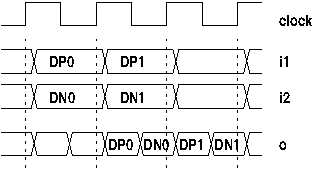
\includegraphics{oddr}
            
            The clock used for the DDR registers is the current clock.
            
            {\bf ce} is an optional clock enable.
            
            {\bf r} can be used to clear the output register and {\bf s} to set
            it to all ones. These can be synchronous or asynchronous depending
            on attribute SRTYPE and are synchronous by default.
            
            No input parameters may contain queue reads.
            
            Example; DDR output, including a clock -

            \begin{lstlisting}[gobble=12, language=threepl]
               str(lvcmos33, "LVCMOS33");

               // package pins
               iopins(out_pins, lvcmos33, "[8]str",
                                   {"F2", "G2", "H2", "J2", "H1", "E1", "G1", "E2"});
               iopins(ddr_clk_pin, lvcmos33, "str", "E17");

               static({out0, out1}, "uint:8");
               
               out0 <- .....;
               out1 <- .....;
               
               value(ddr, "uint:8");
               value(ddr_clk, "log");
               
               oddr(ddr <- out0, out1);
               oddr(ddr_clk <- false, true);
               
               output(,, ddr, loc=out_pins);
               output(,, ddr_clk, loc=ddr_clk_pin);
            \end{lstlisting}
            
            Forwarding a clock via a DDR output is a scheme suggested by
            Xilinx (XAPP 853, p9) to maintain matching phase.



        \subsubsection{oserdes - output serialiser/deserialiser}\label{sec:lposerdes}

            {\bf Library: xilinx/io.3pl}

            {\bf NOT YET IMPLEMENTED!}




    \subsection{library functions}
    
        None.





    \subsection{library classes}
    
        None.
